\section{需求管理}

\subsection{需求管理概述}
需求的影响力贯穿于整个后续的产品生命周期,而不是单纯地存在于需求开发阶段。软件需求规格说明文档要在产品生命周期的各个阶段都扮演重要角色,发挥重要作用。很多后续的开发工作都应该以软件需求规格说明文档的内容为标准和目标来进行。

因此,在需求开发结束之后,还需要有一种力量保证后续的系统开发活动依照需求的基线展开,从而保障系统的质量(质量就是对需求的依从性)。需求管理就是这样的管理活动,它在需求开发之后的产品生命周期当中保证需求作用的有效发挥。

在实践中发现的需求管理的作用有以下几方面:
\begin{itemize}
    \item 增强了项目涉众对复杂产品特征在细节和相互依赖关系上的理解
    \begin{itemize}
        \item 增强了项目涉众对需求(尤其是复杂需求)的掌握
    \end{itemize}
    \item 增进了项目涉众之间的交流
    \begin{itemize}
        \item 减少了可能的误解和交流偏差
    \end{itemize}
    \item 减少了工作量的浪费,提高了生产力
    \begin{itemize}
        \item 需求管理能够更加有效的处理需求的变更
    \end{itemize}
    \item 准确反映项目的状态,帮助进行更好的项目决策
    \begin{itemize}
        \item 需求跟踪信息能够更加准确的反映项目的进展情况
    \end{itemize}
    \item 改变项目文化,使得需求的作用得到重视和有效发挥
    \begin{itemize}
        \item 使得项目涉众认识到需求在项目工作中的重要性
    \end{itemize}
\end{itemize}

需求管理的重要任务有:
\vspace{-0.8em}
\begin{multicols}{2}
    \begin{itemize}
        \item 交流涉众需要什么
        \item 将需求应用、实施到解决方案
        \item 驱动设计和实现工作
        \item 控制变更
        \item 将需求分配到子系统
        \item 测试和验证最终产品
        \item 控制迭代式开发中的变化
        \item 辅助项目管理
    \end{itemize}
\end{multicols}
\vspace{-1em}

\textbf{需求管理的3个活动:维护需求基线、实现需求跟踪和控制变更}
\begin{figure}[H]
	\centering
	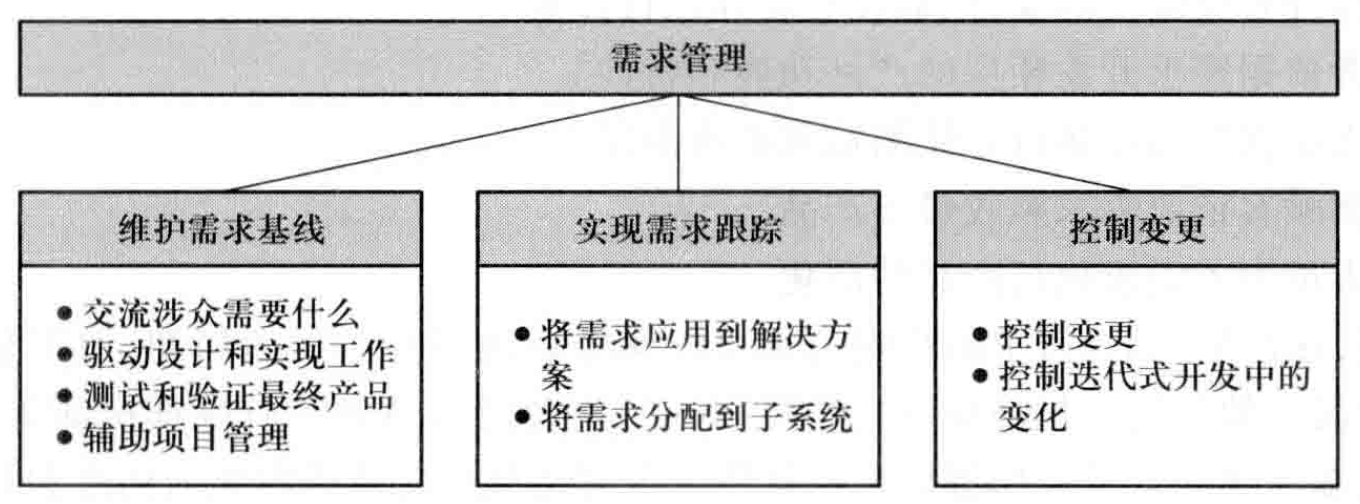
\includegraphics[width=0.7\textwidth]{img/需求管理活动.png}
    \caption*{\textbf{需求管理活动}}
    \vspace{-1em}
\end{figure}


\subsection{维护需求基线}

\subsubsection{需求基线}
[IEEE 1990]定义基线为:已经通过正式评审和批准的规格说明或产品,它可以作为进一步开发的基础,并且只有通过正式的变更控制过程才能修改它
\begin{itemize}
    \item 是被明确和固定下来的需求集合,是项目团队需要在某一特定产品版本中实现的特征和需求集合
\end{itemize}

\begin{figure}[H]
	\centering
    \vspace{-0.5em}
	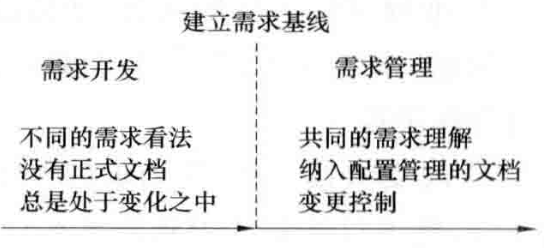
\includegraphics[width=0.5\textwidth]{img/需求基线示意.png}
    \caption*{需求基线示意}
    \vspace{-1em}
\end{figure}


\subsubsection{需求基线的内容}
\vspace{-0.8em}
\begin{multicols}{2}
    \begin{itemize}
        \item 标识符,为后续的项目工作提供一个共同的交流参照
        \item 当前版本号,保证项目的各项工作都建立在最新的一致需求基础之上
        \item 源头,在需要进一步深入理解或者改变需求时,可以回溯到需求的源头
        \item 理由,提供需求产生的背景知识
        \item 优先级,后续的项目工作可以参照优先级进行安排和调度
        \item 状态,交流和具体需求相关的项目工作状况
        \item 成本、工作量、风险、可变性,为需求的设计和实现提供参考信息,驱动设计和实现工作
        {\fangsong
        \item 需求创建的日期
        \item 和需求相关的项目工作人员,包括需求的作者、设计者、实现者、测试者等
        \item 需求涉及的子系统
        \item 需求涉及的产品版本号
        \item 需求的验收和验证标准}
    \end{itemize}
\end{multicols}
\vspace{-1em}


\subsubsection{需求基线的维护}

\paragraph*{配置管理}~{} \par
将需求基线纳入配置管理,它的主要工作有以下几方面
\vspace{-0.8em}
\begin{multicols}{2}
    \begin{itemize}
        \item 标识配置项
        \begin{itemize}
            \item 递增数值,例如1, 2, $\cdots$, $x$
            \item 层次式数值编码,例如1.1.1, 1.2.1, $\cdots$, $x.y.z$;
            \item 层次式命名编码,例如Order.Place.Date, Order.Place.Register, $\cdots$, Task.Step.Substep
        \end{itemize}
        \item 版本控制
        \begin{itemize}
            \item 每一条单独的需求需要进行版本控制
            \item 相关的需求文档也需要进行版本控制
        \end{itemize}
        \item 变更控制
        \item 访问审计
        \begin{itemize}
            \item 记录和审计访问的情况
        \end{itemize}
        \item 状态报告
        \begin{itemize}
            \item 反映需求基线的成熟度(变化的幅度越大,成熟度越低)、稳定性(改变的次数越多,稳定性越差)等
        \end{itemize}
    \end{itemize}
\end{multicols}
\vspace{-1em}

\paragraph*{状态维护}~{} \par
需求的状态可以分为若干种类别(如下表所示),每一种类别都反映和具体需求相关的项目工作的进展状况。因此,只要在项目进展当中及时和准确地维护需求基线内的需求状态,就可以得到项目进展状况的准确反映。
\vspace{-0.8em}
\begin{center}
\begin{longtable}{|m{4cm}<{\centering}|m{9cm}|}
    \hline
    \multicolumn{1}{|c|}{状态} & \multicolumn{1}{c|}{定义}                                                 \\ \hline
    已提议(Proposed)            & 该需求已被有相应权限的人提出                                                          \\ \hline
    已批准(Approved)            & 该需求已经被分析,它对项目的影响已进行了估计,并且已经被分配到某一特定版本的基线中。关键涉众已同意包含这一需求,软件开发团队已承诺实现这一需求 \\ \hline
    已实现(Implemented)         & 实现这一需求的系统组件已经完成了设计和实现。这一需求已经被跟踪到相关的设计元素和实现元素                            \\ \hline
    已验证(Verified)            & 已在集成产品中确认了这一需求的功能实现是正确的。这一需求已经被跟踪到相关的测试用例。这一需求目前可以被认为是已完成了              \\ \hline
    已删除(Deleted)             & 已批准的需求又从需求基线中取消了。要解释清楚为什么要删除这一需求,以及是谁决定删除的                              \\ \hline
    已否决(Rejected)            & 需求已被提议,但并不在下一版本中实现它。要解释清楚为什么要否决这一需求,以及是谁决定否决的                           \\ \hline
\end{longtable}
\end{center}
\vspace{-3.7em}


\subsection{实现需求跟踪}

\subsubsection{需求跟踪}
需求跟踪能避免在开发过程或者演化过程中与需求基线不一致或者偏离的风险,分为前向跟踪和后向跟踪两种
\begin{figure}[H]
	\centering
    \vspace{-0.5em}
	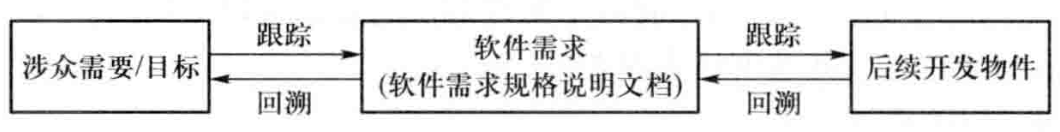
\includegraphics[width=0.7\textwidth]{img/需求跟踪的联系类型.png}
    \caption*{需求跟踪的联系类型}
    \vspace{-1em}
\end{figure}

前向跟踪是指被定义到软件需求规格说明文档之前的需求演化过程
\begin{itemize}
    \item 向前跟踪到需求:说明涉众的需要和目标产生了哪些软件需求
    \item 从需求向后回溯:说明软件需求来源于哪些涉众的需要和目标
\end{itemize}

后向跟踪是指被定义到软件需求规格说明文档之后的需求演化过程
\begin{itemize}
    \item 从需求向前跟踪:说明软件需求是如何被后续的开发物件支持和实现的
    \item 回溯到需求的跟踪:说明各种系统开发的物件是因为什么原因(软件需求)而被开发出来的
\end{itemize}

\subsubsection{需求跟踪的实现方法}
需求跟踪的实现方法主要有矩阵、实体关系模型和交叉引用3种,其中需求跟踪矩阵是最为常用的方法

\begin{table}[H]
    \centering
    \vspace{-0.2em}
    \begin{tabular}{|c|c|c|c|c|}
    \hline
    用户需求  & 功能性需求                & 设计组件          & 实现组件                                                                          & 测试用例                                                                      \\ \hline
    UC-28 & Catalog.query.sort   & Class catalog & Catalog.sort()                                                                & \begin{tabular}[c]{@{}c@{}}Search.7\\ Search.8\end{tabular}               \\ \hline
    UC-29 & Catalog.query.import & Class catalog & \begin{tabular}[c]{@{}c@{}}Catalog.import()\\ Catalog.validate()\end{tabular} & \begin{tabular}[c]{@{}c@{}}Search.12\\ Search.13\\ Search.14\end{tabular} \\ \hline
    \end{tabular}
    \caption*{需求跟踪矩阵示例}
    \vspace{-1em}
\end{table}


\subsubsection{需求跟踪过程的建立}
需求跟踪过程的建立需要考虑下列因素
\vspace{-0.8em}
\begin{multicols}{2}
    \begin{itemize}
        \item 明确需求跟踪需要解决的问题
        \item 说明需求跟踪过程的目标
        \item 明确需要捕获的跟踪联系
        \item 组织提供资源支持和技术支持
        \item 制定有效的过程策略
        \item 便利需求跟踪信息的使用
    \end{itemize}
\end{multicols}
\vspace{-1em}


\subsubsection{需求依赖}
\begin{wraptable}{r}{7.3cm}
    \centering
    \vspace{-1.5em}
    \begin{tabular}{|c|c|c|c|c|c|c|}
        \hline
        依赖 & R1 & R2 & R3 & R4 & R5 & R6 \\ \hline
        R1 &    &    & $\ast$  & $\ast$  &    &    \\ \hline
        R2 &    &    &    &    & $\ast$  & $\ast$  \\ \hline
        R3 &    &    &    & $\ast$  & $\ast$  &    \\ \hline
        R4 &    & $\ast$  &    &    &    &    \\ \hline
        R5 &    &    &    &    &    & $\ast$  \\ \hline
        R6 &    &    &    &    &    &    \\ \hline
    \end{tabular}
    \caption*{依赖联系的需求跟踪矩阵示例}
    \vspace{-3em}
\end{wraptable}

在需求跟踪的各种联系当中,有一种特殊的跟踪联系——需求依赖。大多数的需求并不是完全独立的,它们在一种复杂的机制中互相影响,这就是需求依赖。

需求依赖联系的特殊性并不在于它的重要性,而在于它是难以发现、建立和维护的

需求交互作用管理:用于发现、管理和部署需求之间关键联系的活动

\subsection{需求变更控制}

\subsubsection{需求变化}
需求的变化是正当和不可避免的
\vspace{-0.8em}
\begin{multicols}{3}
    \begin{itemize}
        \item 问题发生了改变
        \item 环境发生了改变
        \item 需求基线存在缺陷
        {\fangsong
        \item 用户变动
        \item 用户对软件的认识变化
        \item 相关产品的出现}
    \end{itemize}
\end{multicols}
\vspace{-1em}


\subsubsection{变更控制过程}
需求变更控制就是以可控、一致的方式进行需求基线中需求的变更处理,包括对变化的评估、协调、批准或拒绝、实现和验证。

\begin{figure}[H]
	\centering
	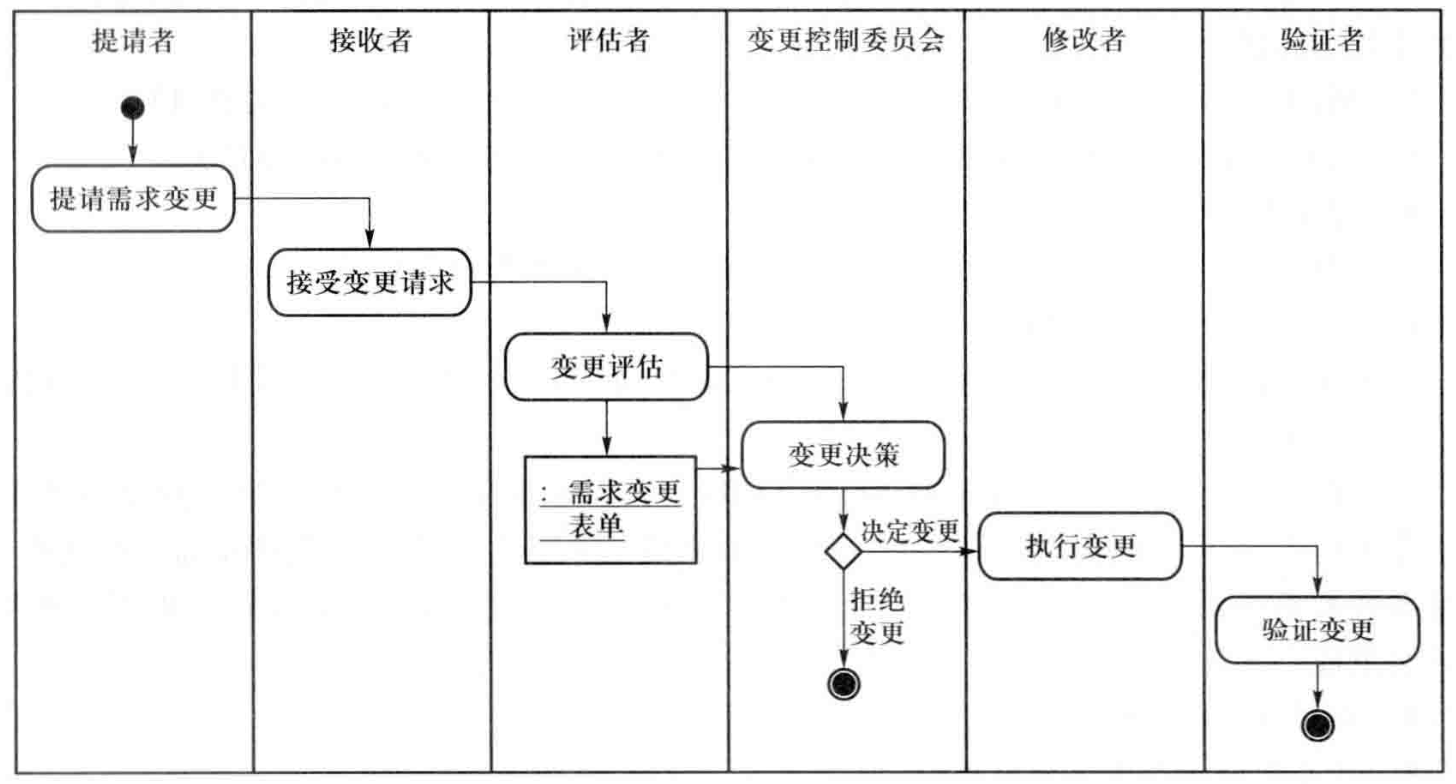
\includegraphics[width=0.85\textwidth]{img/变更控制过程.png}
    \caption*{变更控制过程}
    \vspace{-1em}
\end{figure}

变更评估的内容要以正式文档(如变更请求表单)的方式固定下来, 并提交给变更控制委员会。变更控制委员会(CCB)评价需求的变更,做出批准或者拒绝变化的决定,并确保已批准变化的实现。

\begin{wraptable}{r}{8.6cm}
    \centering
    \vspace{-2em}
    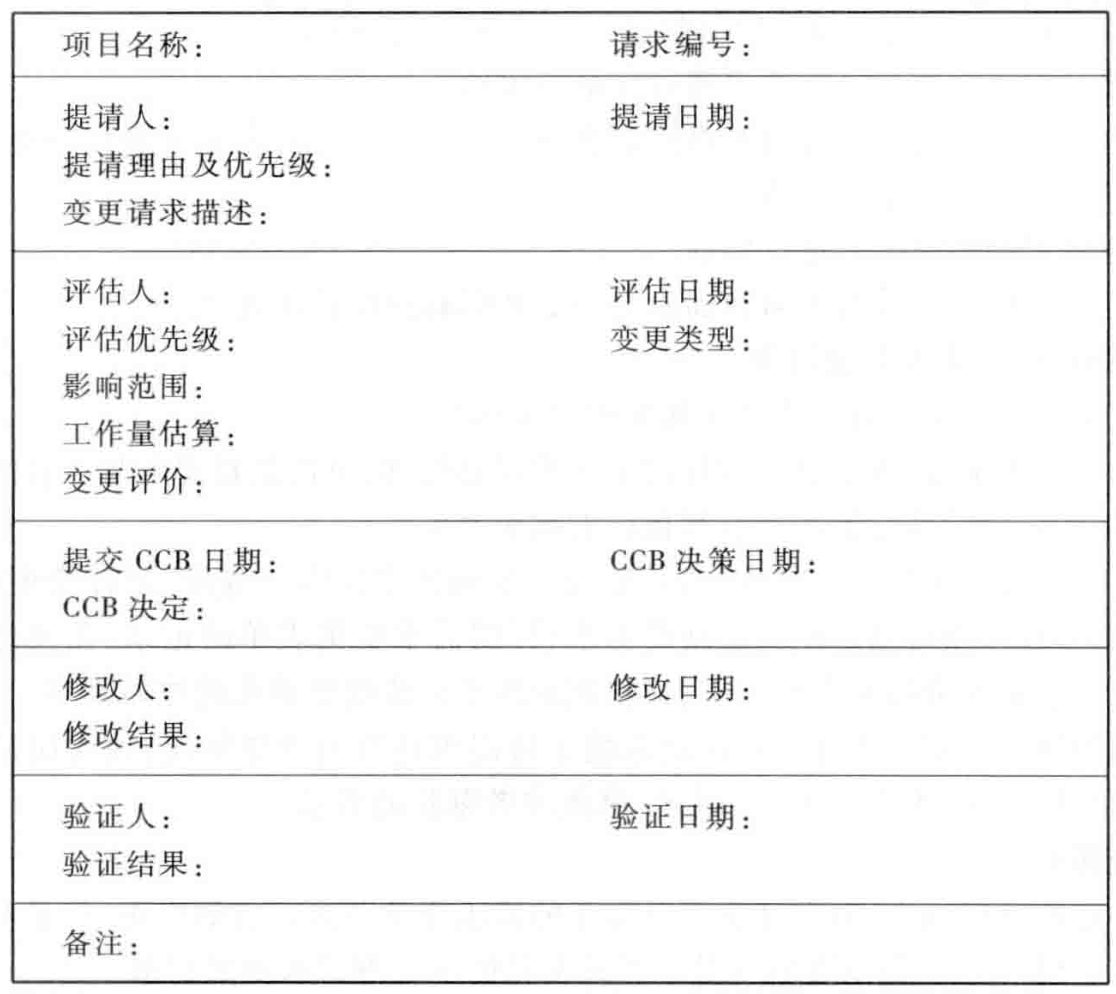
\includegraphics[width=8.5cm]{img/变更请求表单.png}
    \caption*{变更请求表单}
    \vspace{-5em}
\end{wraptable}

变更控制委员会是在项目中成立的一个团队,它的职责是评价需求的变更,做出批准或者拒绝变更的确定,并确保已批准变更的实现。变更控制委员会可能由来自下列部门的人员组成:
\begin{itemize}
    \item 项目或程序管理部门
    \item 产品管理或者需求分析部门
    \item 开发部门
    \item 测试或者质量保障部门
    \item 市场或客户代表
    \item 编写用户文档的部门
    \item 技术支持或帮助部门
    \item 配置管理部门
\end{itemize}

\subsubsection{变更控制中的注意事项}
\textbf{认识到变更的必要性,并为之制定计划}
\begin{itemize}
    \item 定义明确的变更控制过程,建立变更控制的有效渠道
    \item 所有提交的需求变更请求都要进行仔细的评估
    \item 是否进行变更的决定应该由变更控制委员会统一做出
    \item 必须对变更的实现结果进行验证
    \item 需求的变化情况要及时的通知到所有会受到影响的项目涉众
\end{itemize}

\textbf{维护需求基线,审计变更记录}

\textbf{管理范围蔓延}
\begin{itemize}
    \item 根据业务目标、产品前景和项目范围,评估每一项提议的新增需求和特性
\end{itemize}

\textbf{灵活应对变更请求}
\vspace{-0.8em}
\begin{multicols}{2}
    \begin{itemize}
        \item 推迟产品的交付时间
        \item 要求增派人手:在有限的情况下有效
        \item 要求员工加班工作:只能适度的使用
        \item 推迟或者去除尚未实现的优先级较低的需求
        \item 容许产品质量的降低:尽量不使用
    \end{itemize}
\end{multicols}
\vspace{-1em}

\textbf{使用辅助工具}

工具应该具有以下几个特性,以支持需求变更过程:
\vspace{-0.8em}
\begin{multicols}{2}
    \begin{itemize}
        \item 可用定义变更请求中的数据项
        \item 可用辅助项目涉众完成变更控制过程的协作
        \item 可以帮助维护需求基线,审计变更记录
        \item 能够将变更情况及时的通知到相关人员
        \item 可以生成标准的和定制的报告和图表 
    \end{itemize}
\end{multicols}
\vspace{-1em}


